\chapter{分布式系统的基本要素}\label{chap:distributed-system}
\addtocontents{los}{\protect\addvspace{10pt}}

\begin{intro}

\end{intro}

\section{Vector Clock}\label{sec:vector-clock}

\subsection{}

\subsection{}


\section{一致性哈希}\label{sec:consistent-hasing}

本节整理自博客『一致性哈希算法及其在分布式系统中的应用%
\footnote{http://blog.codinglabs.org/articles/consistent-hashing.html}%
』

本节将会从实际应用场景出发,介绍一致性哈希算法(Consistent Hashing)及其在分布式系统中的应用。首先本节会描述一个在日常开发中
经常会遇到的问题场景,借此介绍一致性哈希算法以及这个算法如何解决此问题;接下来会对这个算法进行相对详细的描述,并讨论一些如虚拟节点
等与此算法应用相关的话题。

\subsection{分布式缓存问题}

假设我们有一个网站,最近发现随着流量增加,服务器压力越来越大,之前直接读写数据库的方式不太给力了,于是我们想引入 Memcached
作为缓存机制。现在我们一共有三台机器可以作为 Memcached 服务器,如图 \ref{fig:system-memcached-deployment} 所示。

\begin{figure}[hbtp]
\centering
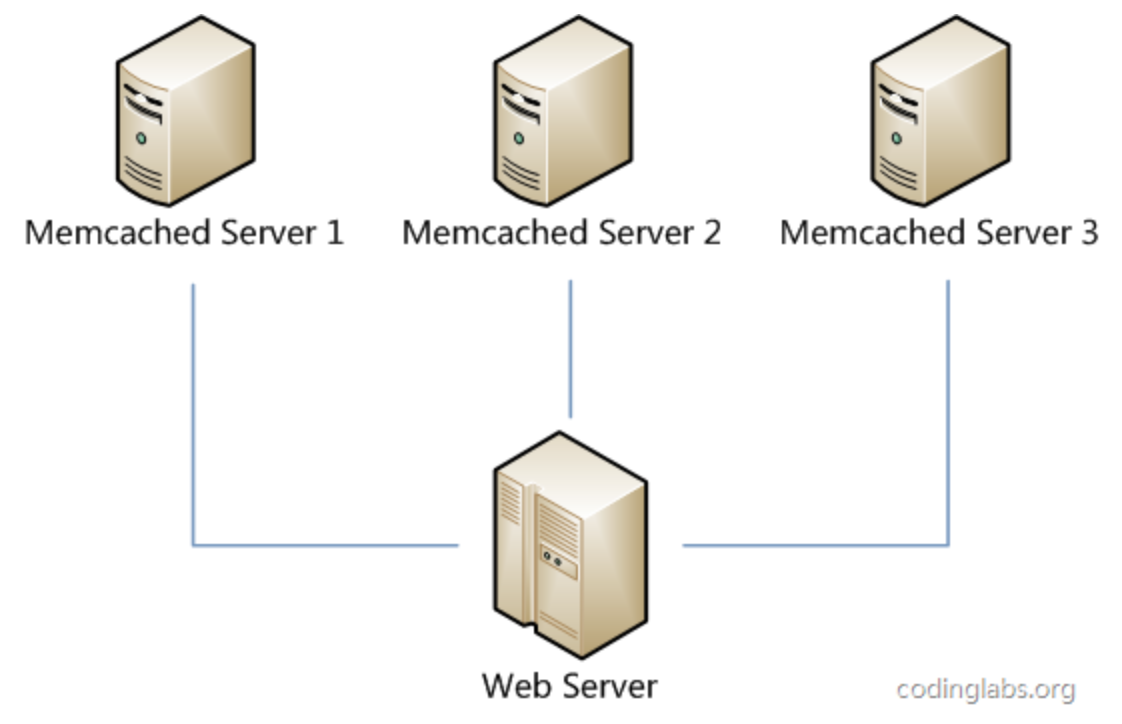
\includegraphics[width=0.45\textwidth]{system-memcached-deployment}
\caption{三台 Memcached 服务器}
\label{fig:system-memcached-deployment}
\end{figure}

很显然,最简单的策略是将每一次 Memcached 请求随机发送到一台 Memcached 服务器,但是这种策略可能会带来两个问题:
\begin{enumerate}
	\item 同一份数据可能被存在不同的机器上而造成数据冗余
	\item 有可能某数据已经被缓存但是访问却没有命中,因为无法保证对相同key的所有访问都被发送到相同的服务器
\end{enumerate}
因此,随机策略无论是时间效率还是空间效率都非常不好。

要解决上述问题只需做到如下一点:保证对相同 key 的访问会被发送到相同的服务器。很多方法可以实现这一点,最常用的方法是计算哈希。
例如对于每次访问,可以按如下算法计算其哈希值:
\begin{equation*}
h = Hash(key) \% 3
\end{equation*}
其中,Hash 是一个从字符串到正整数的哈希映射函数。这样,如果我们将 Memcached Server 分别编号为 0、1、2,那么就可以根据上式和
key 计算出服务器编号 h,然后去访问。

这个方法虽然解决了上面提到的两个问题,但是存在一些其它的问题。如果将上述方法抽象,可以认为通过:
\begin{equation*}
h = Hash(key) \% N
\end{equation*}
这个算式计算每个 key 的请求应该被发送到哪台服务器,其中,N 为服务器的台数,并且服务器按照 0 $\sim$ (N-1) 编号。这个算法的问题在于
容错性和扩展性不好。所谓容错性是指当系统中某一个或几个服务器变得不可用时,整个系统是否可以正确高效运行;而扩展性是指当加入新的
服务器后,整个系统是否可以正确高效运行。

现假设有一台服务器宕机了,那么为了填补空缺,要将宕机的服务器从编号列表中移除,后面的服务器按顺序前移一位并将其编号值减一,
此时每个 key 就要按 $h = Hash(key) \% (N-1)$ 重新计算;同样,如果新增了一台服务器,虽然原有服务器编号不用改变,但是
要按$h = Hash(key) \% (N+1)$重新计算哈希值。因此系统中一旦有服务器变更,大量的 key 会被重定位到不同的服务器从而造成大量的
缓存不命中。而这种情况在分布式系统中是非常糟糕的。

一个设计良好的分布式哈希方案应该具有良好的单调性,即服务节点的增减不会造成大量哈希重定位。一致性哈希算法就是这样一种哈希方案。


\subsection{一致性哈希算法}

\noindent\textbf{算法简述}

一致性哈希算法(Consistent Hashing)最早在这篇论文%
\footnote{Consistent Hashing and Random Trees: Distributed Caching Protocols for Relieving Hot Spots on the World Wide Web}%
中提出。简单来说,一致性哈希将整个哈希值空间组织成一个虚拟的圆环,如假设某哈希函数 H 的值空间为 $0 \sim 2^{32}-1$
(即哈希值是一个 32 位无符号整形),整个哈希空间环如图 \ref{fig:system-hashing-ring-1} 所示。
\begin{figure}[hbtp]
\centering
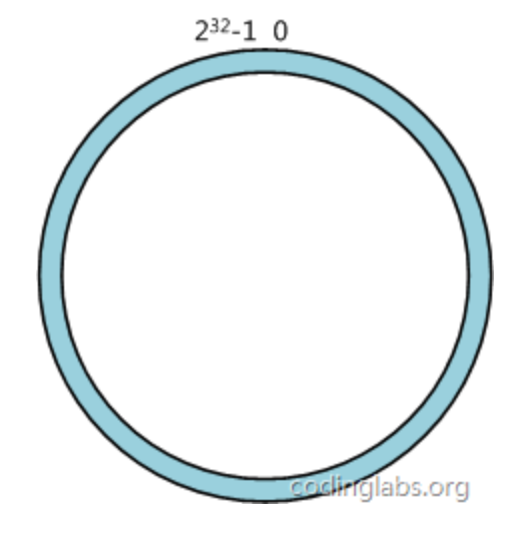
\includegraphics[width=0.3\textwidth]{system-hashing-ring-1}
\caption{哈希空间环}
\label{fig:system-hashing-ring-1}
\end{figure}
整个空间按顺时针方向组织。0 和 $2^{32}-1$ 在零点中方向重合。

下一步将各个服务器使用 H 进行一个哈希,具体可以选择服务器的 ip 或主机名作为关键字进行哈希,这样每台机器就能确定其在哈希环上的位置,
这里假设将上文中三台服务器使用 ip 地址哈希后在环空间的位置如图 \ref{fig:system-hashing-ring-2} 所示

\begin{figure}[hbtp]
\centering
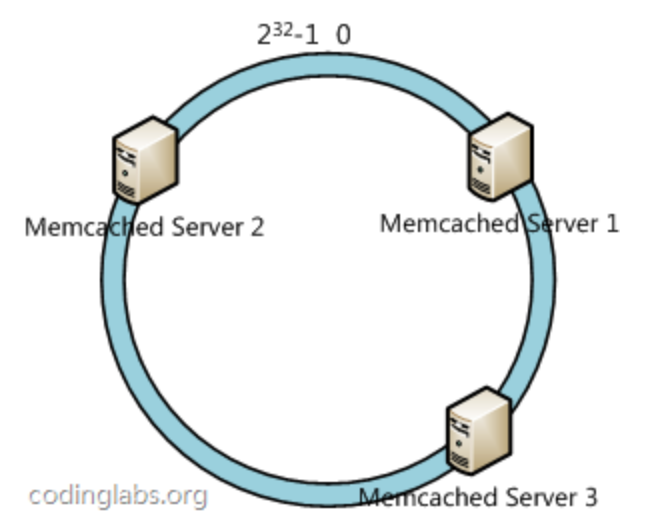
\includegraphics[width=0.3\textwidth]{system-hashing-ring-2}
\caption{三台服务器映射到哈希环上的位置}
\label{fig:system-hashing-ring-2}
\end{figure}

接下来使用如下算法定位数据访问到相应服务器:将数据 key 使用相同的函数 H 计算出哈希值 h,根据 h 确定此数据在环上的位置,从此位置
沿环顺时针『行走』,第一台遇到的服务器就是其应该定位到的服务器。

例如我们有 A、B、C、D 四个数据对象,经过哈希计算后,在环空间上的位置如图 \ref{fig:system-hashing-ring-3}

\begin{figure}[hbtp]
\centering
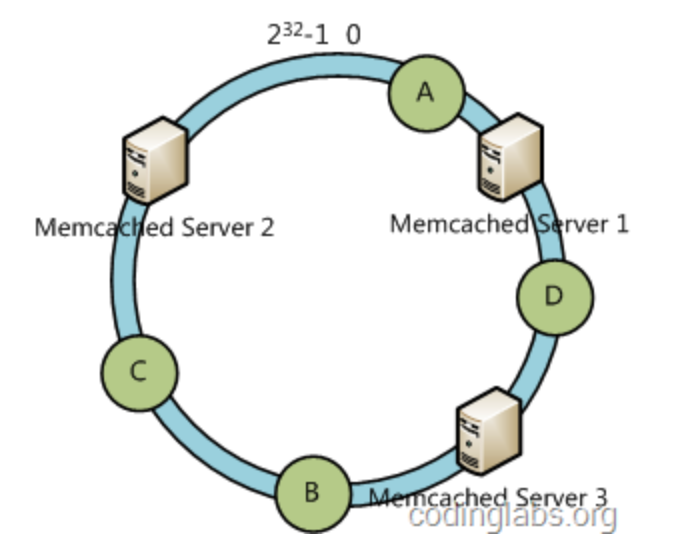
\includegraphics[width=0.3\textwidth]{system-hashing-ring-3}
\caption{四个数据对象映射到哈希环上的位置}
\label{fig:system-hashing-ring-3}
\end{figure}

根据一致性哈希算法,数据 A 会被定位到 Server 1 上,D 被定为到 Server 3 上,而 B、C 分别被定为到 Server 2 上。

\noindent\textbf{容错性与可扩展性分析}

下面分析一致性哈希算法的容错性和可扩展性。现假设 Server 3 宕机了:

\begin{figure}[hbtp]
\centering
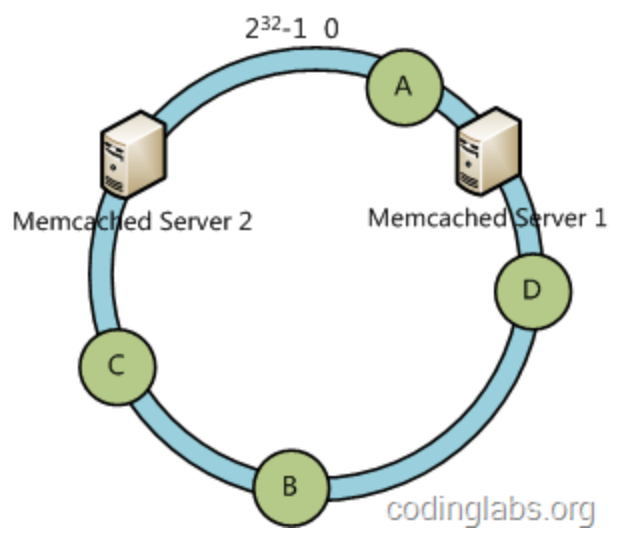
\includegraphics[width=0.3\textwidth]{system-hashing-ring-4}
\caption{Server3宕机}
\label{fig:system-hashing-ring-4}
\end{figure}

可以看到此时 A、C、B 不会受到影响,只有 D 节点被重定位到 Server 2。一般的,在一致性哈希算法中,如果一台服务器不可用,
则受影响的数据仅仅是此服务器到其环空间中前一台服务器(即顺着逆时针方向行走遇到的第一台服务器)之间数据,其它不会受到影响。

下面考虑另外一种情况,如果我们在系统中增加一台服务器 Memcached Server 4:

\begin{figure}[hbtp]
\centering
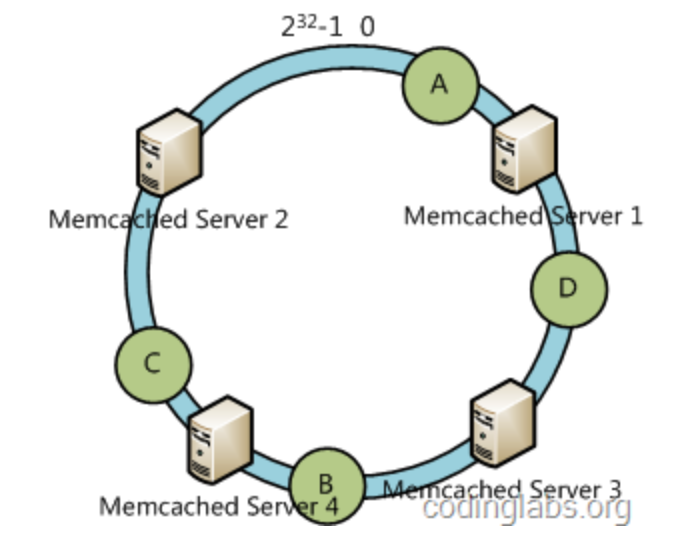
\includegraphics[width=0.3\textwidth]{system-hashing-ring-5}
\caption{增加Server4}
\label{fig:system-hashing-ring-5}
\end{figure}

此时 A、D、C 不受影响,只有 B 需要重定位到新的 Server 4。一般的,在一致性哈希算法中,如果增加一台服务器,则受影响的数据
仅仅是新服务器到其环空间中前一台服务器(即顺着逆时针方向行走遇到的第一台服务器)之间数据,其它不会受到影响。

综上所述,一致性哈希算法对于节点的增减都只需重定位环空间中的一小部分数据,具有较好的容错性和可扩展性。

\noindent\textbf{虚拟节点}

一致性哈希算法在服务节点太少时,容易因为节点分部不均匀而造成数据倾斜问题。例如我们的系统中有两台服务器,其环分布如图%
\ref{fig:system-hashing-ring-6}:

\begin{figure}[hbtp]
\centering
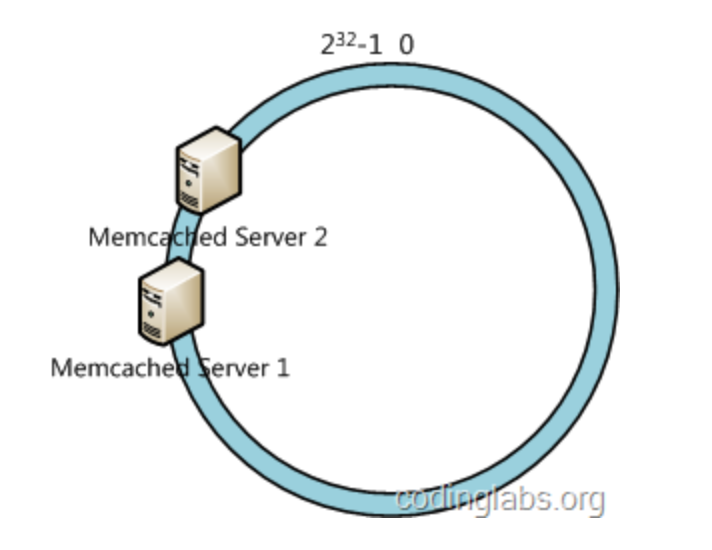
\includegraphics[width=0.3\textwidth]{system-hashing-ring-6}
\caption{节点太少造成的数据倾斜}
\label{fig:system-hashing-ring-6}
\end{figure}

此时必然造成大量数据集中到 Server 1 上,而只有极少量会定位到 Server 2 上。为了解决这种数据倾斜问题,一致性哈希算法引入了
虚拟节点机制,即对每一个服务节点计算多个哈希,每个计算结果位置都放置一个此服务节点,称为虚拟节点。具体做法可以在服务器 ip 或主机名
的后面增加编号来实现。例如上面的情况,我们决定为每台服务器计算三个虚拟节点,于是可以分别计算 “Memcached Server 1\#1”、
“Memcached Server 1\#2”、“Memcached Server 1\#3”、“Memcached Server 2\#1”、“Memcached Server 2\#2”、
“Memcached Server 2\#3” 的哈希值,于是形成六个虚拟节点:

\begin{figure}[hbtp]
\centering
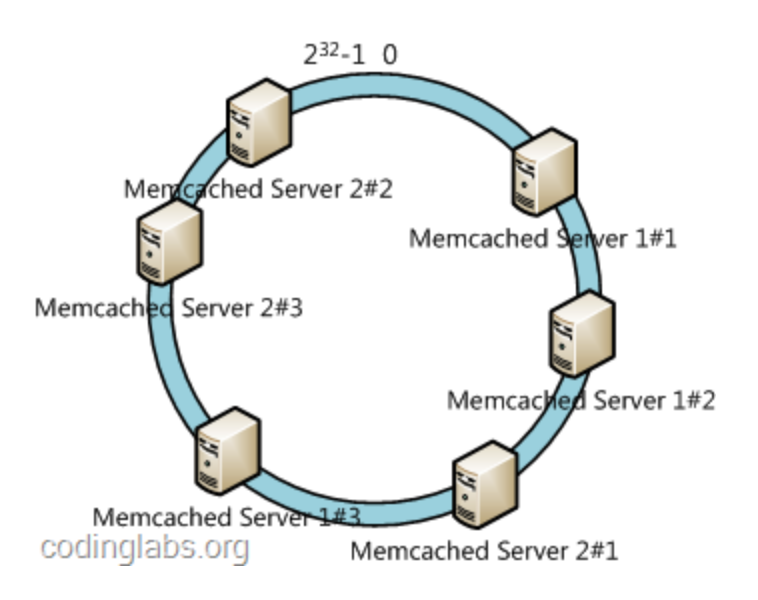
\includegraphics[width=0.3\textwidth]{system-hashing-ring-7}
\caption{使用虚拟节点来实现负载均衡}
\label{fig:system-hashing-ring-7}
\end{figure}

同时数据定位算法不变,只是多了一步虚拟节点到实际节点的映射,例如定位到 “Memcached Server 1\#1”、“Memcached Server 1\#2”、
“Memcached Server 1\#3” 三个虚拟节点的数据均定位到 Server 1 上。这样就解决了服务节点少时数据倾斜的问题。
在实际应用中,通常将虚拟节点数设置为 32 甚至更大,因此即使很少的服务节点也能做到相对均匀的数据分布。

\noindent\textbf{总结}

目前一致性哈希基本成为了分布式系统组件的标准配置,例如 Memcached 的各种客户端都提供内置的一致性哈希支持。本节只是简要介绍了这个算法,
更深入的内容可以参看原论文。














\endinput
